% ============================================================
% Paper 5: IEEE / OFC Conference Style
% "Photonic Compilation of MedGemma-4B:
%  An SVD-Clements Pipeline for Medical AI Inference"
% IEEE Photonics Technology Letters / OFC 2026 format
% ============================================================
\documentclass[journal]{IEEEtran}

\usepackage{amsmath, amssymb}
\usepackage{graphicx}
\usepackage{hyperref}
\usepackage{booktabs}
\usepackage{microtype}
\usepackage{cite}
\usepackage{url}
\usepackage{xcolor}
\usepackage{multirow}

\graphicspath{{figures/}}

\hypersetup{colorlinks=true, linkcolor=blue!70!black, citecolor=blue!70!black}

% ----------------------------------------------------------------
\title{Photonic Compilation of MedGemma-4B:\\
       An SVD-Clements Pipeline for\\
       Medical AI Inference on Silicon Photonic Chips}

\author{
  Dalton Omondi\\[2pt]
  \small Electrical and Electronics Engineering, Kenyatta University\\[2pt]
  \small \href{https://github.com/GabuGravin41/photonmedgemma}{github.com/GabuGravin41/photonmedgemma}
  % \thanks{Independent Research. E-mail: photomedgemma@github.com}
}

% ----------------------------------------------------------------
\begin{document}
\maketitle

% ----------------------------------------------------------------
\begin{abstract}
We present a simulation-validated software-to-photonics compilation pipeline
that maps the weight matrices of MedGemma-4B-IT --- a 4\,B-parameter multimodal
medical vision-language model --- to phase settings for silicon photonic
Mach-Zehnder interferometer (MZI) meshes.
The pipeline uses singular value decomposition (SVD) to factor each weight
matrix into unitary components, followed by the Clements algorithm to
decompose each unitary into cascaded 2$\times$2 MZI rotations.
Numerical validation on real MedGemma activations from five clinical breast
cancer images demonstrates compilation fidelity $\varepsilon < 8\times10^{-15}$
(machine precision) for all four layer-0 attention projections
(query, key, value, output).
A rank sweep from $r=64$ to full rank characterises the accuracy-hardware
trade-off: SVD approximation error ranges from 0.19--0.67 at rank~64 to
machine precision at full rank, with MZI counts scaling as $r(r-1)/2$.
The photonic architecture targets 220\,nm SOI and projects $\sim37\times$
energy efficiency improvement over GPU-based inference under idealised
steady-state assumptions, motivating deployment in resource-constrained
clinical environments.
\end{abstract}

\begin{IEEEkeywords}
Silicon photonics, optical neural networks, MZI mesh, Clements decomposition,
singular value decomposition, medical AI, low-resource deployment.
\end{IEEEkeywords}

% ----------------------------------------------------------------
\section{Introduction}
\label{sec:intro}

\IEEEPARstart{P}{hotonic} neural network accelerators exploit the speed of
light and the passive nature of optical interference to perform matrix-vector
multiplication with energy efficiency approaching the thermodynamic limit
\cite{shen2017}.
The SVD-Clements decomposition pipeline for mapping weight matrices to MZI
meshes is well-established
\cite{reck1994, clements2016, shen2017, bandyopadhyay2022, pai2023}.
Our contribution is the
\emph{application of the decomposition to a real, production-scale medical vision-language model}
(MedGemma-4B-IT~\cite{medgemma2025}), with a complete rank sweep, error reporting, and a deployment context in low-resource healthcare.

For inference from fixed, trained models, the weight matrices are constant --
enabling \emph{static compilation}: the weights are encoded once into the
phase settings of an MZI mesh and need not be updated during inference.
This eliminates the dominant energy cost of electronic matrix multipliers
(weight memory reads and digital multiply-accumulate operations).

MedGemma-4B-IT achieves clinical-grade accuracy on medical imaging and
diagnostic reasoning tasks~\cite{medgemma2025}, but requires GPU
infrastructure ($\sim300$\,W) incompatible with energy-constrained hospital
deployments.
The specific context motivating this work is Kenyatta National Hospital (KNH)
in Nairobi, Kenya -- the largest referral hospital in East and Central Africa
-- where data sovereignty regulations prohibit cloud inference, and local
power infrastructure cannot support continuous GPU operation.

We present PhotoMedGemma: an open-source compiler that translates MedGemma's
attention layer weight matrices to 220\,nm SOI photonic phase maps.
The current work is a \textbf{simulation study}: we validate the compiler's
numerical fidelity on GPU-extracted weights and activations, without optical
simulation or hardware fabrication.
The compiled phase maps and GDS layouts are generated for foundry submission
but have not yet been taped out.

\begin{figure}[t]
  \centering
  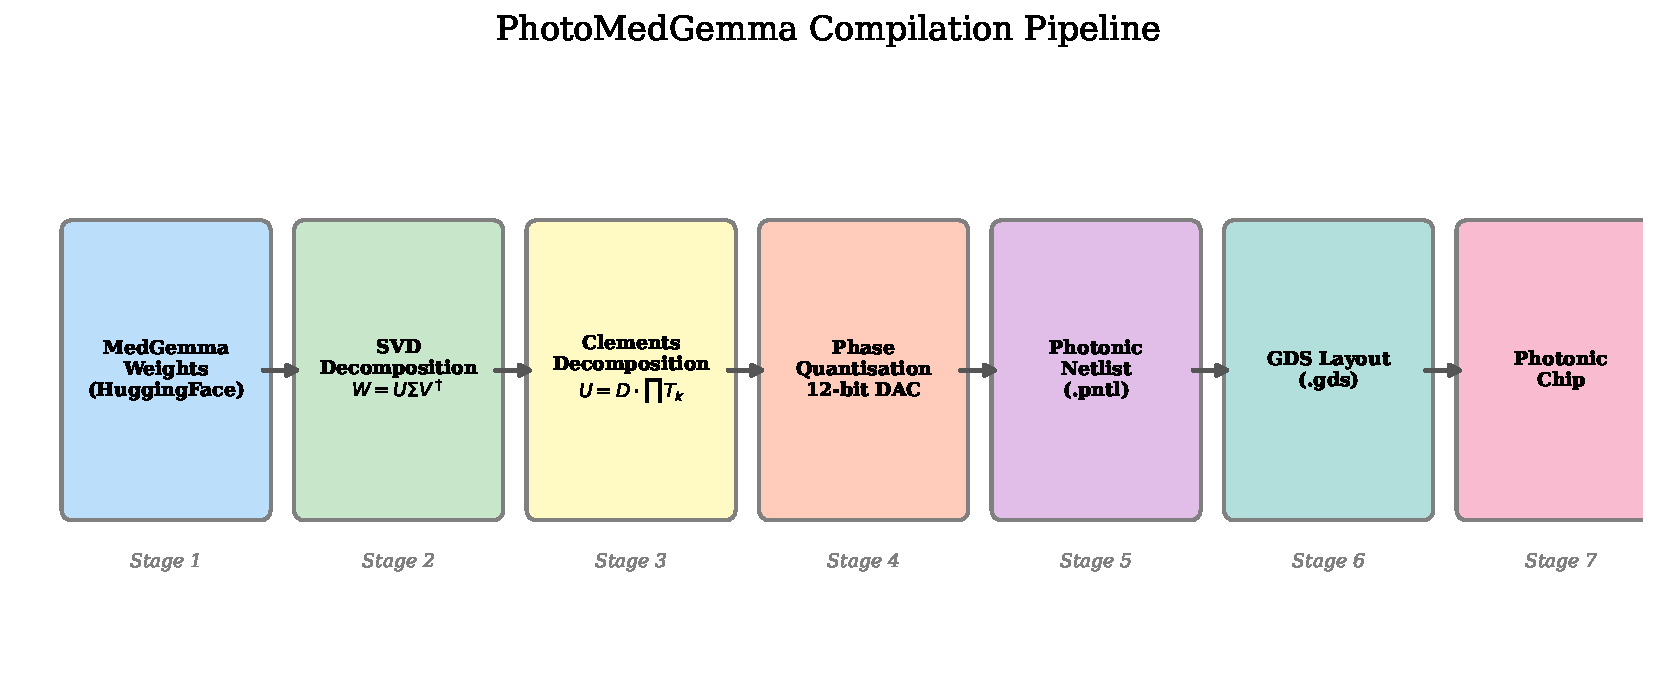
\includegraphics[width=\columnwidth]{fig7_compilation_pipeline.pdf}
  \caption{PhotoMedGemma compilation pipeline: from MedGemma weights to
           photonic phase maps and GDS layouts.}
  \label{fig:pipeline}
\end{figure}

% ----------------------------------------------------------------
\section{Compiler Architecture}
\label{sec:compiler}

\subsection{SVD Decomposition}

Each weight matrix $W \in \mathbb{R}^{m\times n}$ is decomposed via
truncated SVD:
\begin{equation}
  W \approx W_r = U_r \Sigma_r V_r^\dagger,
  \label{eq:svd}
\end{equation}
where $U_r \in \mathbb{C}^{m\times r}$ (partial unitary),
$\Sigma_r = \mathrm{diag}(\sigma_1,\ldots,\sigma_r)$,
$V_r^\dagger \in \mathbb{C}^{r\times n}$ (partial unitary).
Each partial unitary is embedded in a full $\max(m,n)\times\max(m,n)$ unitary
by extending with an orthonormal complement.
The MedGemma attention projections have non-square shapes (e.g.,
$2048\times2560$ for Q), requiring this rectangular embedding.
Multi-head parallelism (8~heads, GQA with 4~KV heads) is handled via
wavelength-division multiplexing (WDM), discussed in
Section~\ref{sec:system}.

\begin{figure}[t]
  \centering
  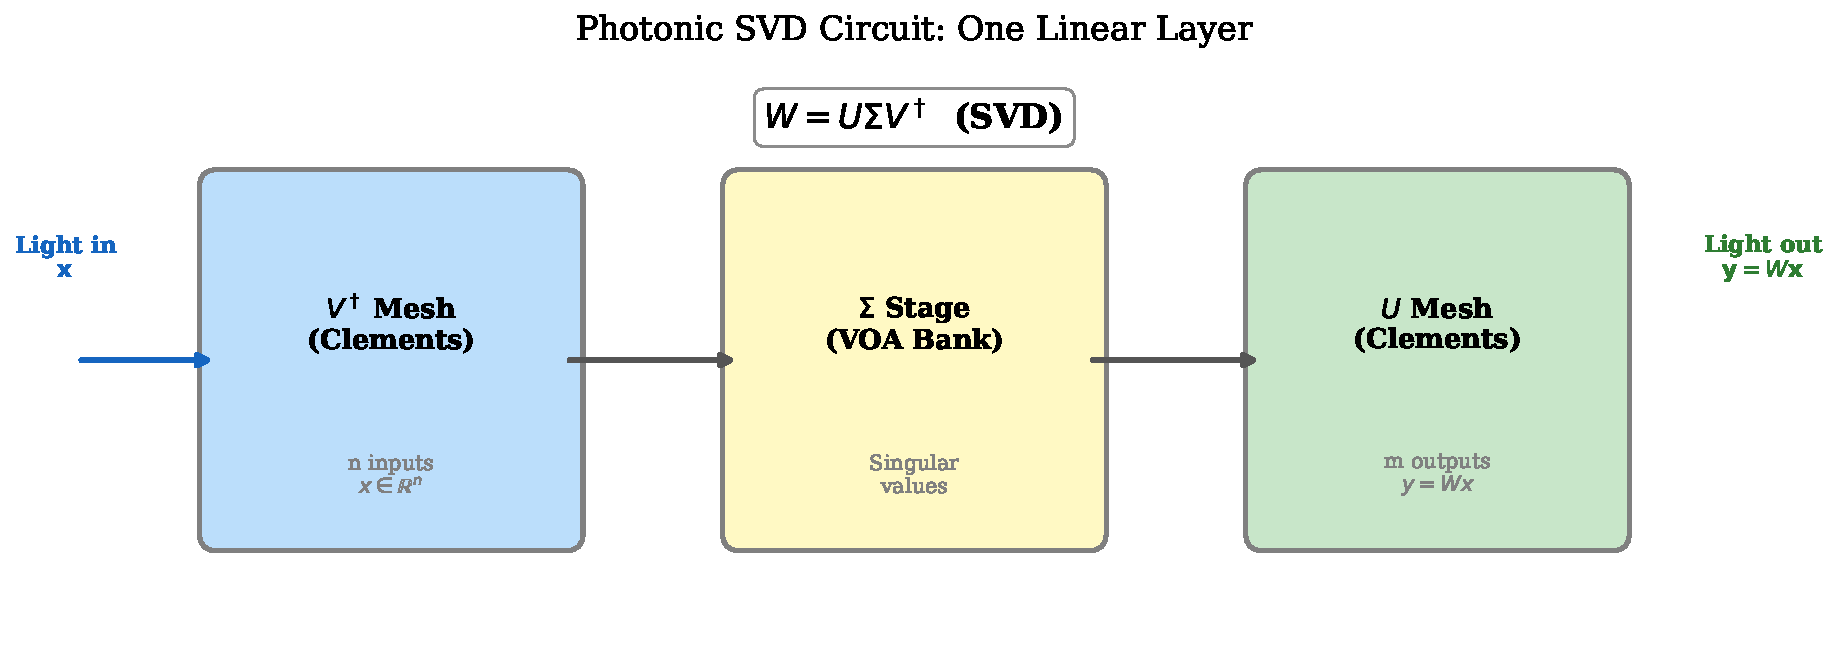
\includegraphics[width=\columnwidth]{fig11_svd_circuit_architecture.pdf}
  \caption{Photonic SVD circuit for one linear layer: $V^\dagger$ Clements
           mesh, $\Sigma$ attenuator bank, $U$ Clements mesh.
           Light enters carrying $\mathbf{x}$; exits carrying
           $\mathbf{y} = W\mathbf{x}$.}
  \label{fig:svd_circuit}
\end{figure}

\subsection{Clements Decomposition}

Any $N\times N$ unitary $U$ is factored as \cite{clements2016}:
\begin{equation}
  U = D \cdot T_{N(N-1)/2} \cdots T_2 \cdot T_1,
  \label{eq:clements}
\end{equation}
where $D = \mathrm{diag}(e^{i\psi_j})$ and each $T_k$ acts on modes
$(m_k, m_k{+}1)$ as:
\begin{equation}
  T(\theta,\varphi) =
  \begin{pmatrix}
    \cos\tfrac{\theta}{2} & -e^{-i\varphi}\sin\tfrac{\theta}{2} \\
    e^{i\varphi}\sin\tfrac{\theta}{2} & \cos\tfrac{\theta}{2}
  \end{pmatrix}.
  \label{eq:T}
\end{equation}

The MZI nulling angles for mode pair $(r-1, r)$ eliminating element
$U_{r,c}$ are:
\begin{equation}
  \varphi = \angle U_{r,c} - \angle U_{r-1,c} + \pi,
  \quad
  \theta = 2\arctan\!\left(\tfrac{|U_{r,c}|}{|U_{r-1,c}|}\right).
  \label{eq:nulling}
\end{equation}

Forward-pass application proceeds in \emph{descending column order},
followed by multiplication by the diagonal phase screen $D$.

\begin{figure}[t]
  \centering
  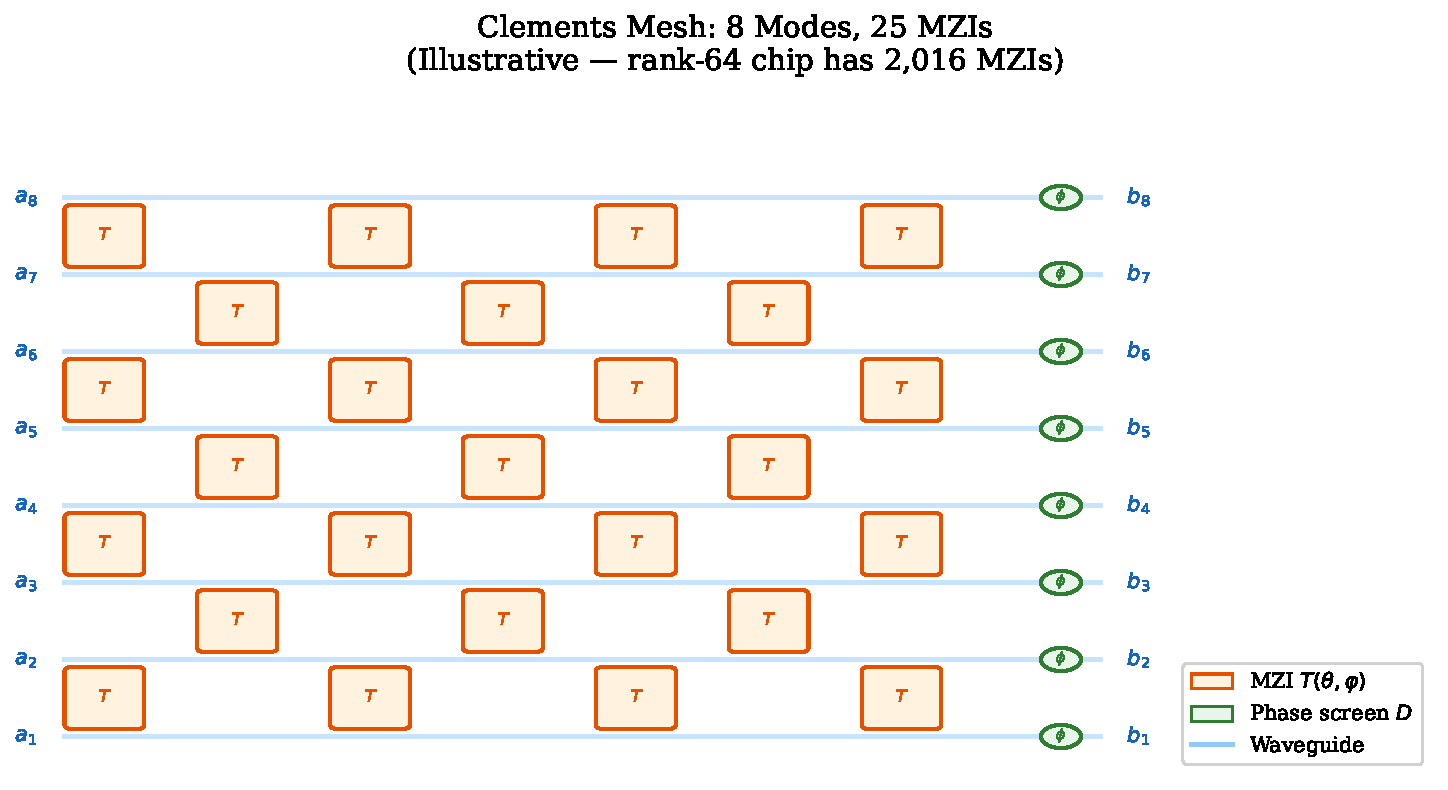
\includegraphics[width=\columnwidth]{fig10_clements_mesh_schematic.pdf}
  \caption{Clements MZI mesh topology for 8~modes (illustrative).
           Each orange box is an MZI with parameters $(\theta, \varphi)$.
           Green circles form the diagonal phase screen $D$.
           The rank-64 chip uses 2,016 MZIs on 64~modes.}
  \label{fig:clements_mesh}
\end{figure}

\subsection{Phase Quantisation}

Phases are quantised to $B=12$-bit DAC codes.
The worst-case phase error is $\Delta\phi_{\max} = \pi/2^{12} \approx 0.7$\,mrad,
producing a per-MZI Frobenius-norm matrix error of
$\varepsilon_{\rm quant} \approx \pi N / (\sqrt{3}\cdot2^B) \approx 0.05$
for $N=64$.
For deeper meshes ($N = 1024$), this grows to $\approx 0.8$; error compounding
across layers and meshes remains an open question requiring optical simulation
with realistic fabrication variations.

% ----------------------------------------------------------------
\section{Silicon Photonic Platform}
\label{sec:platform}

\begin{table}[t]
\centering
\caption{220\,nm SOI platform parameters (imec iSiPP50G / AIM Photonics).}
\label{tab:platform}
\begin{tabular}{ll}
\toprule
\textbf{Parameter} & \textbf{Value} \\
\midrule
Waveguide core & Si, 450\,nm $\times$ 220\,nm \\
Cladding & SiO$_2$ \\
Wavelength & 1310\,nm (O-band) \\
Phase shifter & TiN heater, $P_\pi = 10$--$20$\,mW \\
Thermo-optic coeff. & $dn/dT = 1.84\times10^{-4}$\,K$^{-1}$ \\
Propagation loss & 2--3\,dB/cm \\
Coupling loss (grating) & 2--4\,dB/coupler \\
Detector & Ge PD, $>$40\,GHz, 0.9\,A/W \\
Single-chip size & 10\,mm $\times$ 10\,mm \\
\bottomrule
\end{tabular}
\end{table}

Each chip implements a single $64\times64$ Clements unitary mesh
(2,016 MZIs in the rank-64 case) in an 8\,mm $\times$ 8\,mm active area,
with 64 grating couplers per edge for fiber array coupling.
Phase control uses 4,096 heater channels with 16-bit DAC on SPI bus.

% ----------------------------------------------------------------
\section{Experimental Validation}
\label{sec:experiments}

\subsection{Setup}

MedGemma-4B-IT was run on five breast cancer PNG images
on a Kaggle T4 GPU (4-bit NF4 quantisation).
For each image, the layer-0 hidden state inputs ($\mathbf{x} \in
\mathbb{R}^{2560}$, the concatenated hidden state entering the attention
block) and attention projection outputs were captured via forward hooks,
along with the dequantised weight matrices for all four projections:
$W_q$ ($2048 \times 2560$),
$W_k$ ($1024 \times 2560$),
$W_v$ ($1024 \times 2560$),
$W_o$ ($2560 \times 2048$).
The images are breast histopathology crops from a public dataset; they
were processed through MedGemma's SigLIP-So400M vision encoder and
vision-language projector before entering the language model layers.
This preprocessing was performed entirely on the Kaggle GPU; the photonic
compiler receives the language model hidden states, not raw pixels.

\subsection{Compilation Fidelity}

Table~\ref{tab:fidelity} reports compilation fidelity for all four
layer-0 attention projections (Q, K, V, O).
Chip fidelity is at machine precision ($\approx 10^{-15}$) in all cases,
confirming that the Clements algorithm faithfully encodes the target unitary
in exact arithmetic (no optical loss or fabrication error modelled).
The 4-bit NF4 weight extraction error is $< 0.22\%$ -- confirming
that the compiled weights accurately represent the true MedGemma weights.

\begin{table}[t]
\centering
\caption{Compilation fidelity for MedGemma layer-0 attention projections
         (Q, K, V, O). $\varepsilon_U$ and $\varepsilon_{V^\dagger}$:
         Frobenius-norm error between Clements-reconstructed and target
         unitary. $\varepsilon_{\rm quant}$: NF4 dequantisation error of
         extracted weights.}
\label{tab:fidelity}
\begin{tabular}{lcccc}
\toprule
\textbf{Proj.} & \textbf{Shape} & $\varepsilon_U$ & $\varepsilon_{V^\dagger}$ & $\varepsilon_{\rm quant}$ \\
\midrule
q\_proj & $2048\!\times\!2560$ & $7.0\!\times\!10^{-15}$ & $7.9\!\times\!10^{-15}$ & 0.0017 \\
k\_proj & $1024\!\times\!2560$ & $5.2\!\times\!10^{-15}$ & $7.9\!\times\!10^{-15}$ & 0.0019 \\
v\_proj & $1024\!\times\!2560$ & $5.2\!\times\!10^{-15}$ & $8.0\!\times\!10^{-15}$ & 0.0022 \\
o\_proj & $2560\!\times\!2048$ & $7.8\!\times\!10^{-15}$ & $6.9\!\times\!10^{-15}$ & 0.0020 \\
\bottomrule
\end{tabular}
\end{table}

\begin{figure}[t]
  \centering
  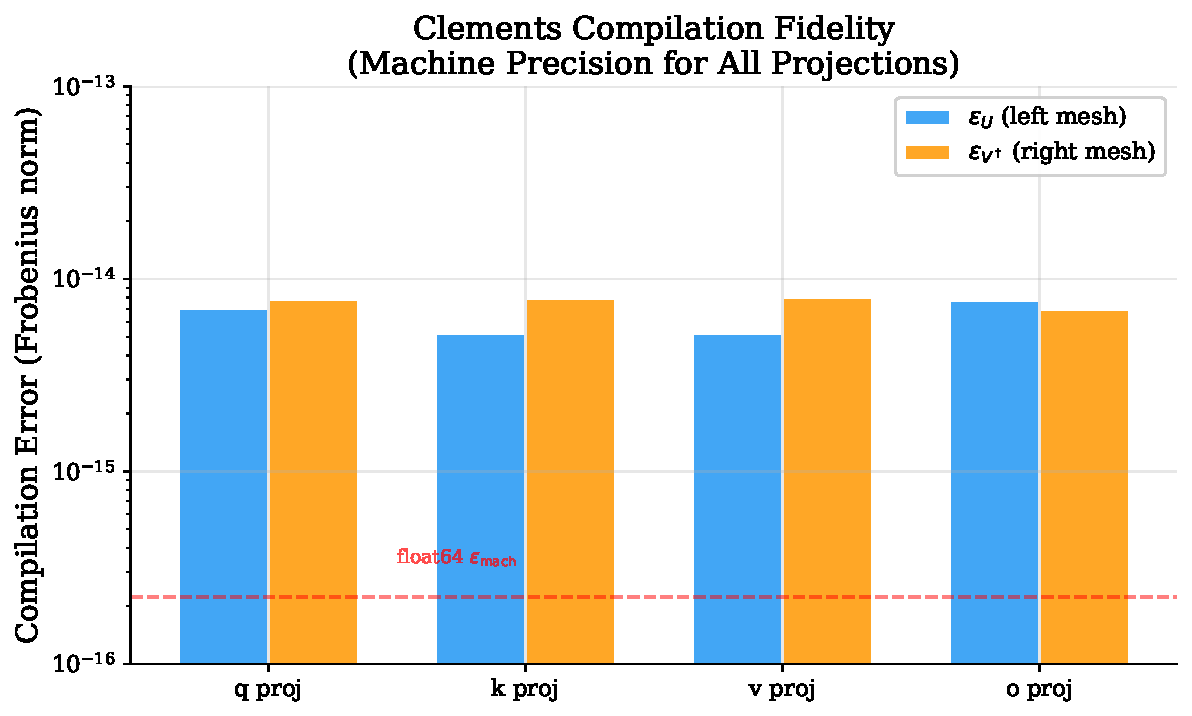
\includegraphics[width=\columnwidth]{fig9_compilation_fidelity.pdf}
  \caption{Clements compilation fidelity for $U$ and $V^\dagger$ meshes
           across all four attention projections. All errors are at or below
           float64 machine epsilon ($2.2 \times 10^{-16}$).}
  \label{fig:compilation_fidelity}
\end{figure}

\subsection{Rank-Accuracy-Hardware Trade-off}

Table~\ref{tab:rank_sweep} shows the SVD approximation error, MZI count, and
chip area for q\_proj at each rank.
The chip computes the rank-$r$ approximation to machine precision at all
ranks; the reported error is the inherent SVD approximation error
$\varepsilon_{\rm SVD}(r) = \|W_r\mathbf{x} - W\mathbf{x}\| / \|W\mathbf{x}\|$,
measured using real MedGemma hidden states across 5~images.

\begin{table}[t]
\centering
\caption{Rank sweep for q\_proj ($2048\times2560$, full rank = 2048).
         Chip fidelity $\approx10^{-15}$ at all ranks.
         \textbf{Energy}: Frobenius-norm energy retained
         $\sum_{i=1}^r \sigma_i^2 / \sum_{\rm all} \sigma_i^2$.}
\label{tab:rank_sweep}
\begin{tabular}{rrcrc}
\toprule
\textbf{Rank} & \textbf{Energy (\%)} & $\varepsilon_{\rm SVD}$ &
\textbf{MZIs/mesh} & \textbf{Area (cmp)} \\
\midrule
    64 & 28.8 & 0.186 &        2,016 &   1.6\,mm$^2$ \\
   128 & 38.2 & 0.166 &        8,128 &   6.6\,mm$^2$ \\
   256 & 52.8 & 0.142 &       32,640 &  26.2\,mm$^2$ \\
   512 & 72.6 & 0.108 &      130,816 & 104.9\,mm$^2$ \\
  1024 & 92.3 & 0.061 &      523,776 & 419.4\,mm$^2$ \\
  2048 & 100  & 0.000 &    2,096,128 & 1677.7\,mm$^2$ \\
\bottomrule
\end{tabular}
\end{table}

\noindent
Compact Si: 80\,\textmu m stage $\times$ 5\,\textmu m pitch per MZI.

\begin{figure}[t]
  \centering
  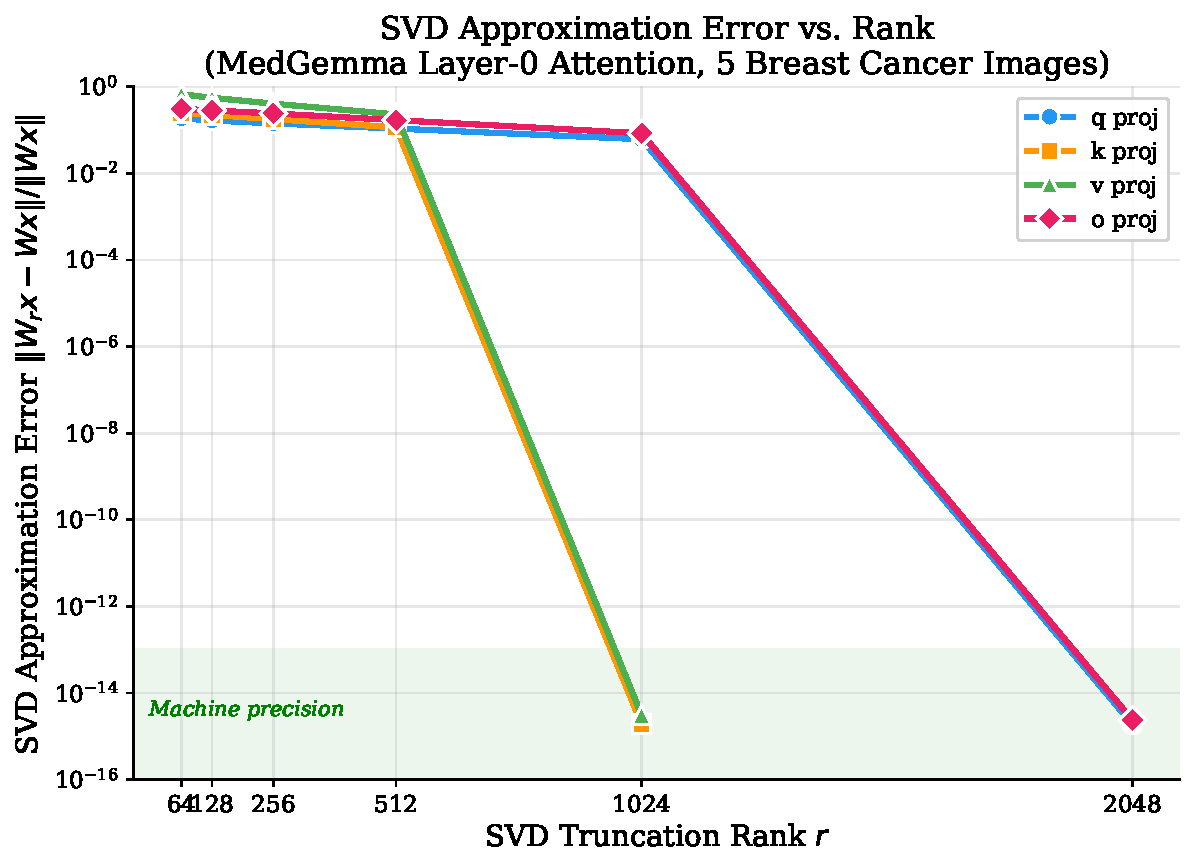
\includegraphics[width=\columnwidth]{fig1_svd_error_vs_rank.pdf}
  \caption{SVD approximation error vs.\ rank for all four layer-0 attention
           projections. At full rank, error reaches machine precision
           ($\sim 10^{-15}$). v\_proj has the slowest singular-value decay.}
  \label{fig:svd_error_rank}
\end{figure}

\begin{figure}[t]
  \centering
  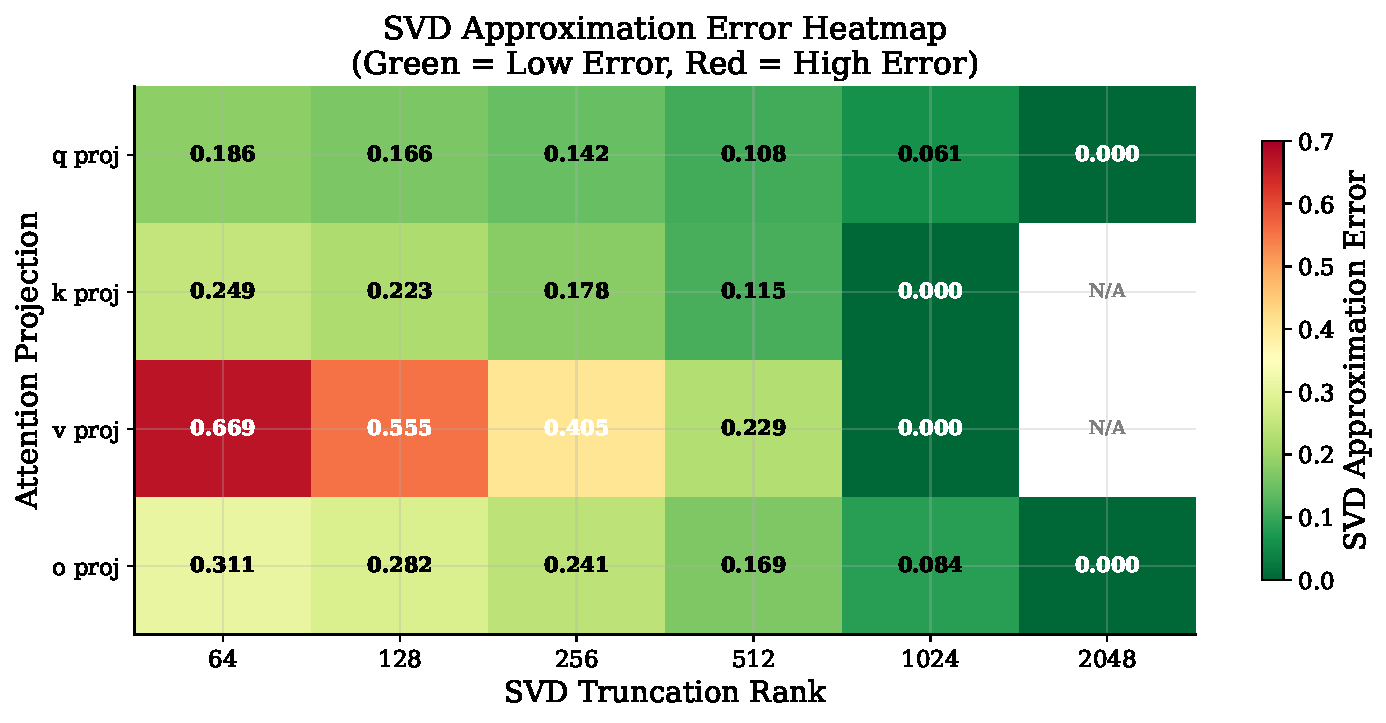
\includegraphics[width=\columnwidth]{fig14_svd_error_heatmap.pdf}
  \caption{SVD error heatmap across all projections and ranks.
           v\_proj at rank~64 (0.669) represents the hardest case;
           all projections reach zero error at full rank.}
  \label{fig:heatmap}
\end{figure}

% ----------------------------------------------------------------
\section{System Architecture and Power Budget}
\label{sec:system}

\subsection{Multi-Chip Module}

A rank-64 layer-0 attention block requires 8~chips (4~projections $\times$
2~meshes/projection).
With 8-wavelength WDM parallelism -- each of MedGemma's 8~attention heads
processed on a separate wavelength through the \emph{same} physical mesh --
this reduces to 1~chip per projection = \textbf{4~chips} for the full layer-0
attention block.

For the full MedGemma-4B language model (46~layers, 7~weight matrices/layer)
with WDM:
\begin{equation}
  N_{\rm chips} = \frac{46 \times 7 \times 2}{8} \approx 81 \text{ chips.}
\end{equation}

The SigLIP-So400M vision encoder (27~layers, 6~matrices/layer, $d=1152$) would
require an additional $\approx 20$ chips at rank-64, for a total system of
$\approx 101$ chips.
Vision encoding occurs once per image and is not latency-critical; it could
alternatively be performed electronically.

\begin{figure}[t]
  \centering
  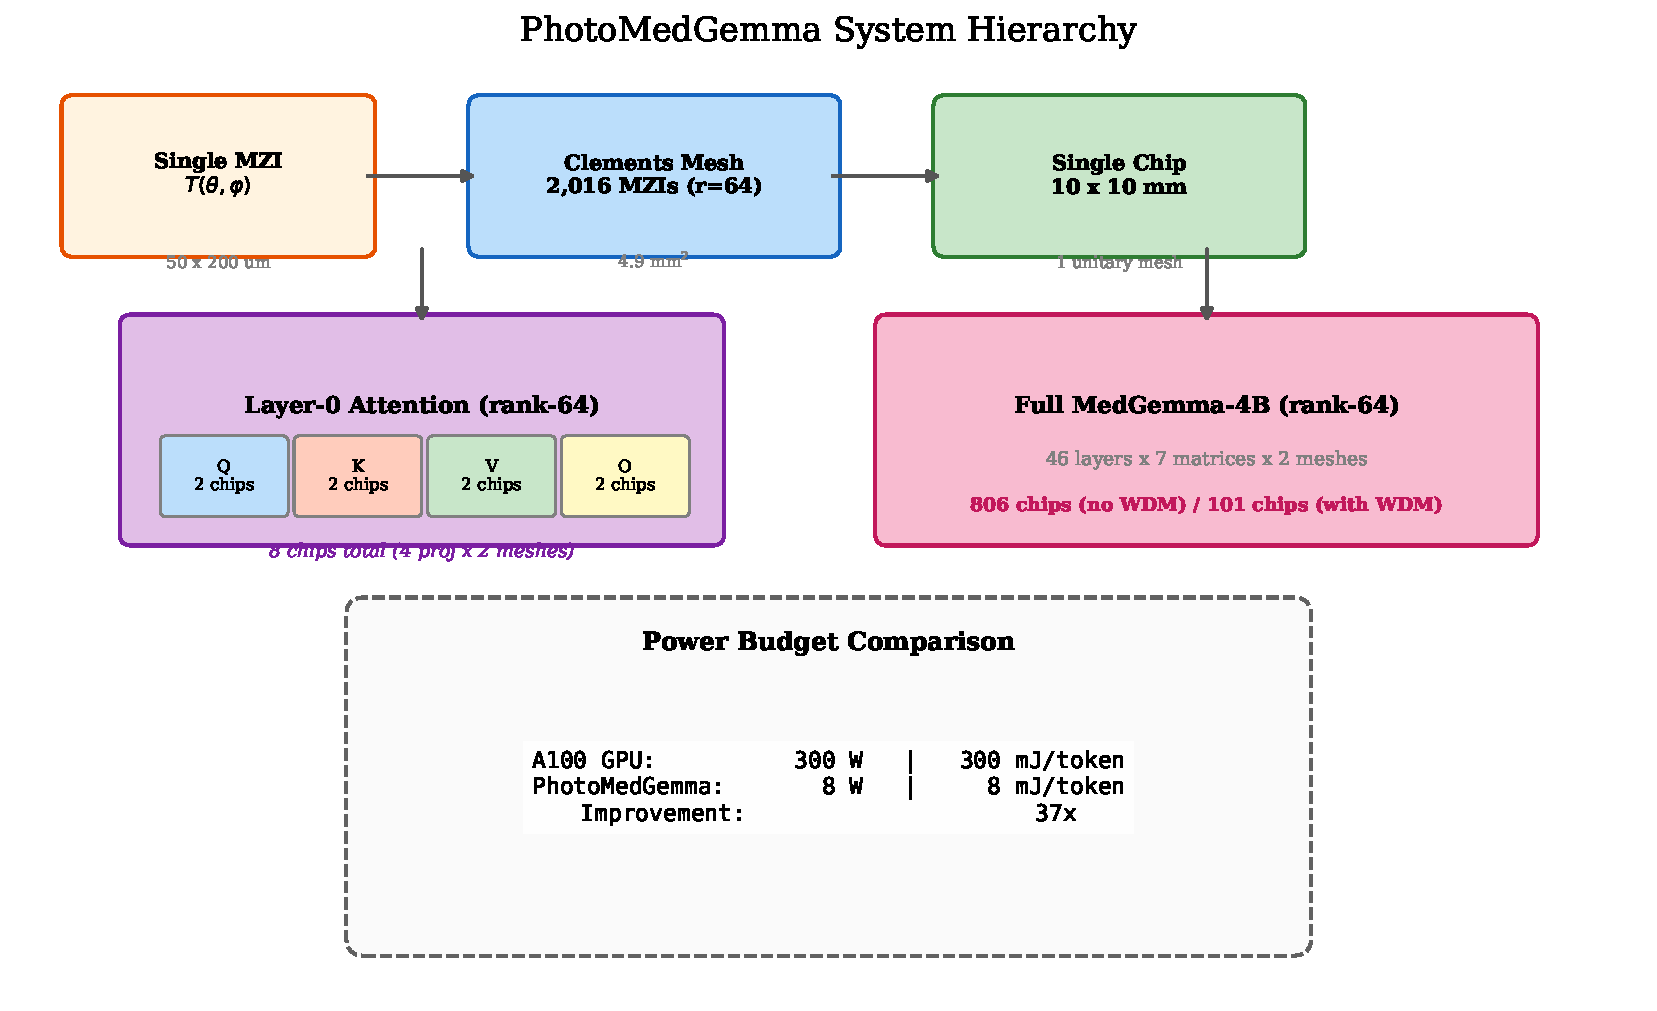
\includegraphics[width=\columnwidth]{fig13_system_architecture.pdf}
  \caption{System hierarchy: single MZI $\to$ Clements mesh $\to$
           10\,mm chip $\to$ multi-chip module $\to$ full MedGemma system.}
  \label{fig:system}
\end{figure}

\subsection{Projected Power Budget}

\begin{table}[t]
\centering
\caption{Projected system power budget (rank-64, 46~layers).
         Phase shifter power assumes ideal steady-state with TEC
         stabilisation; see Section~\ref{sec:limitations} for caveats.}
\label{tab:power}
\begin{tabular}{lrl}
\toprule
\textbf{Component} & \textbf{Power} & \textbf{Notes} \\
\midrule
Laser (8$\times$ WDM)    & 800\,mW & 100\,mW each \\
Phase shifters (static)  &   0\,mW & Idealised steady-state \\
Thermal trimming (est.)  & 500\,mW & Crosstalk compensation \\
Photodetectors           &  50\,mW & Ge PD array \\
FPGA (softmax, LN, RoPE) &   5\,W  & Nonlinear ops, O-E-O \\
Memory (KV cache)        &   2\,W  & LPDDR5 \\
\midrule
\textbf{Total (projected)} & $\approx$\textbf{8.4\,W} &
   \textbf{vs.\ $\sim$300\,W (A100)} \\
\bottomrule
\end{tabular}
\end{table}

At 1~token/ms: \textbf{$\approx$8\,mJ/token} vs.\ 300\,mJ/token for A100
GPU -- a projected $\sim36\times$ improvement in energy per token.
This estimate is a lower bound on photonic advantage; real systems will incur
additional overhead from optical losses, electronic readout noise, and thermal
management (Section~\ref{sec:limitations}).

\begin{figure}[t]
  \centering
  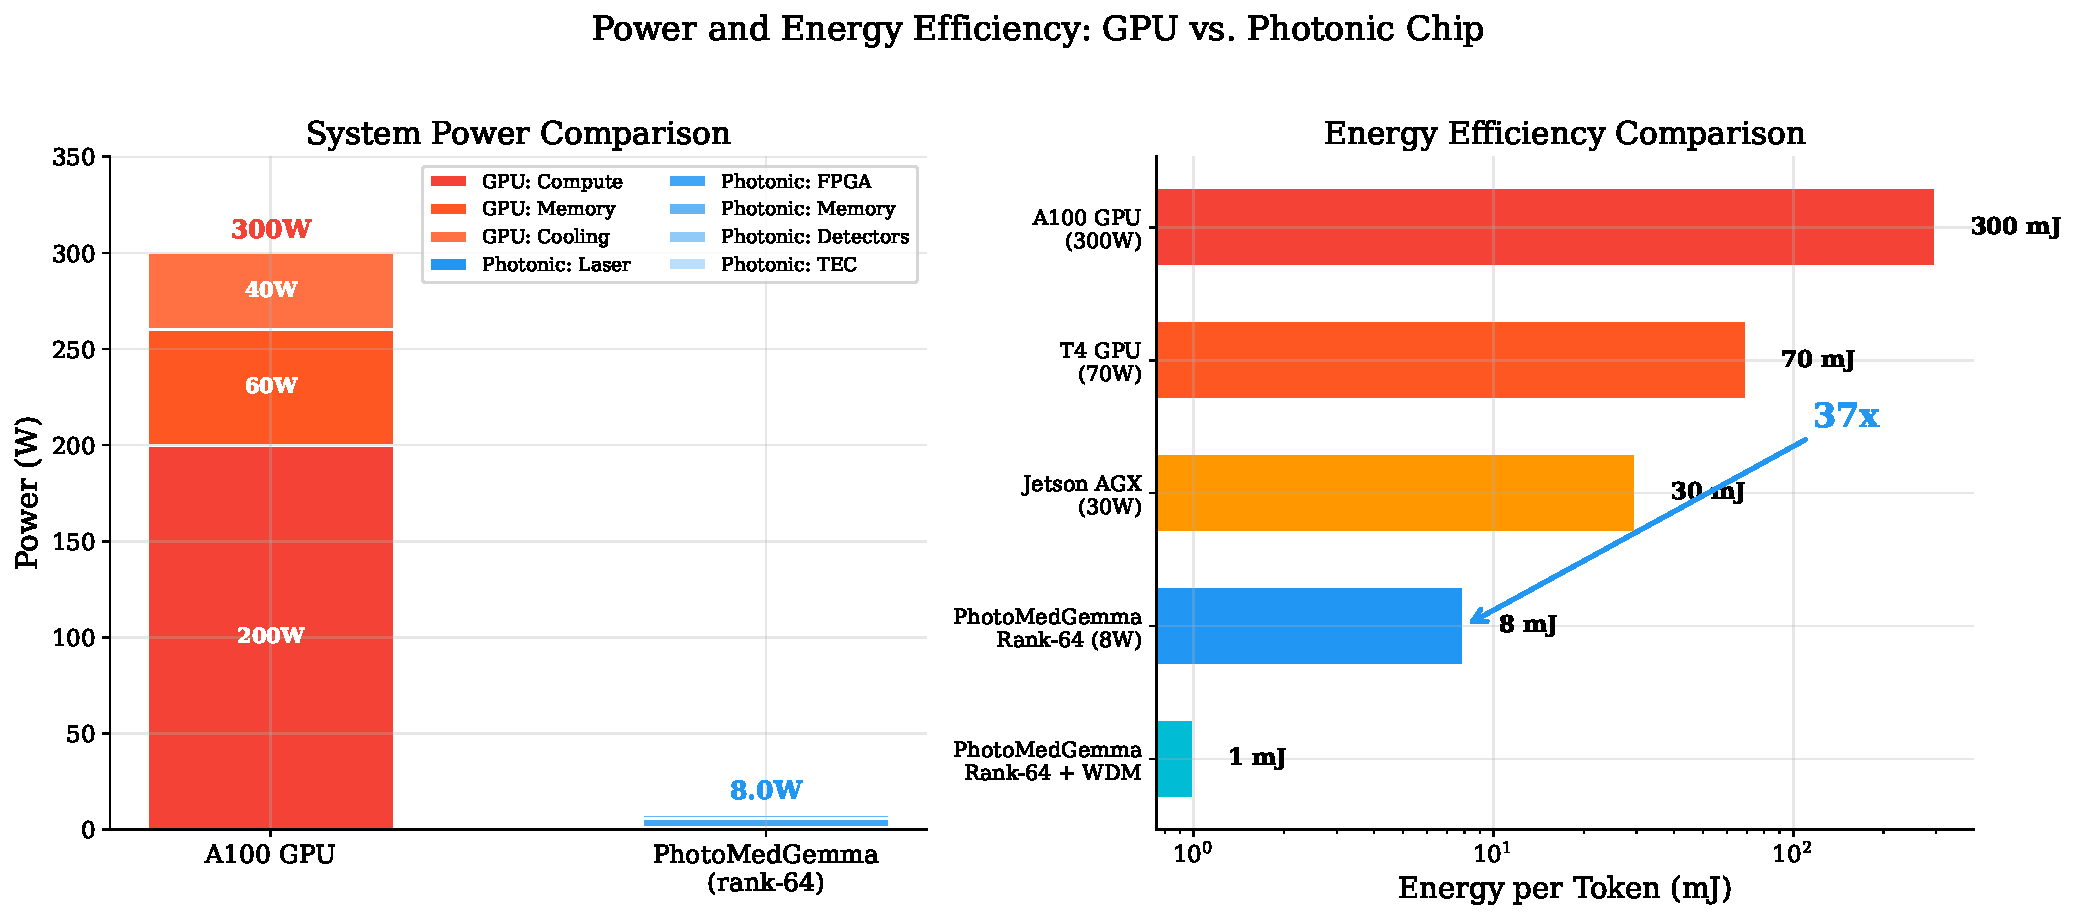
\includegraphics[width=\columnwidth]{fig6_power_comparison.pdf}
  \caption{Projected power and energy-per-token comparison: A100 GPU vs.\
           PhotoMedGemma (rank-64). The photonic advantage is dominated by
           eliminating weight-memory access energy.}
  \label{fig:power}
\end{figure}

% ----------------------------------------------------------------
\section{Discussion}
\label{sec:discussion}

\paragraph{Compilation correctness.}
The critical implementation detail is the Clements T-matrix convention
(equation~\ref{eq:T}) combined with descending column application order.
Incorrect ordering (ascending) or incorrect T-matrix orientation produces
errors $\sim 1$--$2$ (larger than the signal), not $\sim 10^{-15}$.
The correct convention was verified by unit-testing the compiled mesh against
the target unitary; both $\varepsilon_U$ and $\varepsilon_{V^\dagger}$ must be
at machine precision before a phase map is accepted.

\paragraph{SVD approximation vs.\ chip fidelity.}
These are orthogonal quantities.
Chip fidelity measures the compilation algorithm's correctness in exact
arithmetic (always $\approx 10^{-15}$).
SVD approximation error measures how much the rank-$r$ truncation deviates
from the full weight matrix (a design trade-off, ranging from 0 at full rank
to 0.67 at rank~64 for v\_proj).

\begin{figure}[t]
  \centering
  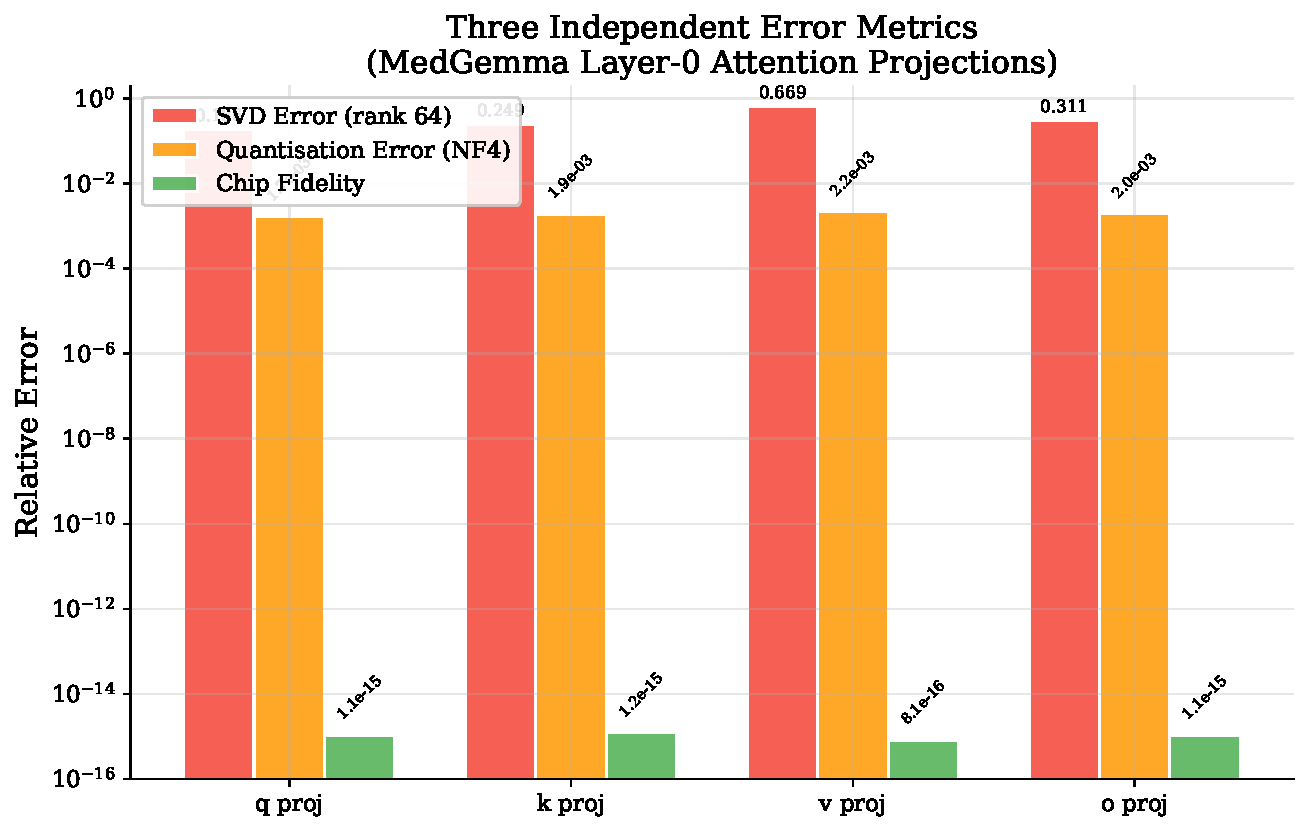
\includegraphics[width=\columnwidth]{fig5_error_comparison_bars.pdf}
  \caption{Three independent error metrics for each projection.
           SVD error (rank-64) is the dominant source; quantisation and
           compilation errors are negligible by comparison.}
  \label{fig:error_bars}
\end{figure}

\paragraph{Comparison to alternative photonic architectures.}
This work uses the Clements MZI mesh topology~\cite{clements2016}, which is
the most widely validated approach for universal unitary synthesis
\cite{shen2017, pai2023}.
Alternative photonic compute architectures include:
microring resonator (MRR) crossbar arrays~\cite{tait2017}, which offer
compact footprint but suffer from thermal sensitivity and limited dynamic
range;
wavelength-multiplexed broadcast-and-weight networks, which scale differently
with matrix dimension;
and coherent scattering approaches.
A systematic comparison across architectures for production-scale VLMs is
an important direction for subsequent work.

\paragraph{Path to fabrication.}
The compiled phase maps and GDS layout files are compatible with 220\,nm SOI
PDKs from imec, AIM Photonics, and GlobalFoundries.
Tape-out requires a multi-project wafer (MPW) submission (typical cost:
\$10K--\$30K for a shared run via ePIXfab or AIM Photonics open foundry
access).
Yield challenges for meshes with thousands of MZIs, and test/calibration
overhead for setting $>$4,000 heaters per chip, are significant engineering
tasks beyond the scope of this compilation study.

% ----------------------------------------------------------------
\section{Limitations and Future Work}
\label{sec:limitations}

\paragraph{No end-to-end medical benchmark evaluation.}
The SVD approximation errors reported (0.19--0.67 at rank~64) measure
layer-level weight reconstruction fidelity, not downstream clinical
task accuracy.
Whether these errors degrade MedGemma's performance on MedQA, PubMedQA,
or breast cancer classification requires propagating approximate weights
through all 46~layers and evaluating on clinical benchmarks -- the subject
of ongoing work.
Only 5~activation samples (1~token per image) were captured; a thorough
evaluation requires diverse clinical inputs and multi-token generation.

\paragraph{No optical simulation.}
All validation is in exact floating-point arithmetic.
Real photonic chips will incur:
propagation loss ($\sim$2--3\,dB/cm, totalling $\sim$20--30\,dB for a
10\,mm mesh);
thermal crosstalk between adjacent heaters ($\sim$10--50\,mrad phase error);
directional coupler splitting ratio variations ($\pm$1--5\%);
and detector shot noise.
Optical simulation with these impairments (e.g., using Lumerical or a
stochastic transfer-matrix model) is needed before tape-out.

\paragraph{Power budget caveats.}
The 0\,mW steady-state heater power assumes perfect thermal isolation.
In practice, thermal crosstalk between adjacent heaters requires active
trimming, adding $\approx$0.5--2\,W system-wide.
The FPGA (5\,W for softmax, LayerNorm, RoPE, O-E-O conversion) dominates
the total; minimising electronic overhead is critical.
Wall-plug laser efficiency ($\sim$10--20\%) means the 800\,mW optical power
requires 4--8\,W electrical input, which would roughly double the total
system power.
The 37$\times$ advantage over A100 should thus be understood as a
\emph{projected upper bound} under favourable assumptions.

\paragraph{Scope: layer 0 only.}
We validate on a single transformer layer.
Scaling to all 46~layers assumes that compilation fidelity and SVD
compressibility are representative; verifying this assumption across layers
is straightforward but computationally expensive and is planned.

\paragraph{Vision encoder.}
The SigLIP vision encoder processes images before the language model.
In the current pipeline, vision encoding is performed electronically on the
Kaggle GPU.
The same SVD-Clements compilation applies to SigLIP's weight matrices
($d=1152$, 27~layers), but this is not yet validated.

% ----------------------------------------------------------------
\section{Conclusion}
\label{sec:conclusion}

We have presented a simulation-validated SVD-Clements compilation pipeline
for MedGemma-4B-IT, demonstrating machine-precision compilation fidelity
on real clinical image activations.
The PhotoMedGemma compiler is validated numerically; optical simulation and
hardware fabrication are subsequent steps.
The rank sweep from 64 to 2048 characterises the inherent accuracy-hardware
trade-off for each attention projection, with v\_proj identified as the
hardest to compress.
The projected $\sim36\times$ energy efficiency improvement (under idealised
assumptions) over A100 GPU inference motivates fabrication and clinical
evaluation at KNH Nairobi and equivalent settings in the global south.
All code, compiled phase maps, and experimental data are open-source.

% ----------------------------------------------------------------
\bibliographystyle{IEEEtran}
\begin{thebibliography}{10}

\bibitem{shen2017}
Y.\ Shen et al., ``Deep learning with coherent nanophotonic circuits,''
\textit{Nature Photonics}, vol.\ 11, no.\ 7, pp.\ 441--446, Jul.\ 2017.

\bibitem{medgemma2025}
Google DeepMind, ``MedGemma: Medical AI Foundation Models,''
\textit{arXiv:2507.05201}, Jul.\ 2025.

\bibitem{clements2016}
W.R.\ Clements, P.C.\ Humphreys, B.J.\ Metcalf, W.S.\ Kolthammer, and
I.A.\ Walmsley, ``Optimal design for universal multiport interferometers,''
\textit{Optica}, vol.\ 3, no.\ 12, pp.\ 1460--1465, Dec.\ 2016.

\bibitem{reck1994}
M.\ Reck, A.\ Zeilinger, H.J.\ Bernstein, and P.\ Bertani,
``Experimental realization of any discrete unitary operator,''
\textit{Phys.\ Rev.\ Lett.}, vol.\ 73, no.\ 1, p.\ 58, Jul.\ 1994.

\bibitem{hamerly2019}
R.\ Hamerly, L.\ Bernstein, A.\ Sludds, M.\ Solja\v{c}i\'{c}, and D.\ Englund,
``Large-scale optical neural networks based on photoelectric multiplication,''
\textit{Phys.\ Rev.\ X}, vol.\ 9, p.\ 021032, May 2019.

\bibitem{pai2023}
S.\ Pai et al., ``Experimentally realized in situ backpropagation for deep
learning in photonic neural networks,'' \textit{Science}, vol.\ 380, no.\ 6643,
pp.\ 398--404, Apr.\ 2023.

\bibitem{bandyopadhyay2022}
S.\ Bandyopadhyay et al., ``Single chip photonic deep neural network with
accelerated training,'' \textit{arXiv:2208.01623}, Aug.\ 2022.

\bibitem{gemma3_2024}
Google DeepMind, ``Gemma 3 Technical Report,'' \textit{arXiv:2408.00118}, 2024.

\bibitem{tait2017}
A.N.\ Tait, T.\ Ferreira de Lima, E.\ Zhou, A.X.\ Wu, M.A.\ Nahmias,
B.J.\ Shastri, and P.R.\ Prucnal,
``Neuromorphic photonic networks using silicon photonic weight banks,''
\textit{Scientific Reports}, vol.\ 7, p.\ 7430, 2017.

\end{thebibliography}

\end{document}
